\section*{Testdesign}
\label{Testdesign}
%
Følgende afsnit vil belyse de forskellige aspekter af feltundersøgelsen fra hvilke spørgsmål der stilles i interviewet for at få testpersonerne til at beskrive deres oplevelse med robotten, rollefordelingen samt hvilke testpersoner, der tilstræbes at rekruttere til hvor testen afvikles og med hvilket udstyr samt fremgangsmåden.  

\subsection*{Testperson}
\label{Testpersoner}
%
I forbindelse med miniprojektet omkring \textit{Descriptive Analysis} vælges det er inddrage naive testpersoner, som derfor ikke får træning i at beskrive deres oplevelse ud fra specifikke termer eller parametre. De naive testpersoner vil derfor være dem der "finder" ordene, som beskriver stimuli - interaktionen med robotten.

Testpersonerne, de rejsende, bliver rekrutteret direkte i Aalborg Lufthavn i området efter sikkerhedskontrollen. Det er som udgangspunkt robotten, der står får rekrutteringen ved at henvende sig til de rejsende med spørgsmålet: \textit{Jeg kommer fra Aalborg Universitet. Må jeg hjælpe dig med at finde rundt i Aalborg Lufthavn?}, har den rejsende lyst til at deltage vil robotten føre dem igennem nogle foruddefineret brugsscenarier, såsom at finde toiletfaciliteter, information om gate og lignende. Fordelen ved at få robotten til at rekruttere testpersoner er, at testpersonerne får et upåvirket førstehåndsindtryk af robotten, som det vil være tilfældet første gang de oplever robotten i lufthavnen. \blankline 
%
Det tilstræbes, at foretage underøgelsen på både kvinder og mænd, gerne med forskellige aldre og rejseformål; forretningsrejse eller ferierejse, hvis muligt vil det ydermere bestræbes at inddrage førstegangs rejsende. Derudover er det et krav, at den rejsende er dansktalende for at undgå, at vigtige pointer går tabt i oversættelsen, når data efterfølgende skal behandles. Antallet af testpersoner er ikke forudbestemt, da undersøgelsen i stedet afsluttes, når der opnåes mætning, hvorved der ikke indsamles ny viden. Dette vurderes af de tilstede værende gruppemedlemmer. Det forventes dog, at udføre undersøgelsen på minimum fem testpersoner.


\subsection*{Interview}
\label{Interview}
%
Efter testpersonen har angivet hvad robotten skal hjælpe med i lufthavnen vil robotten bede testpersonen om at følge efter robotten, istedet for at robotten følger testpersonen hen til det angivne sted følges testpersonen til et interview. Igennem interviewet vil testpersonerne blive stilt nogle spørgsmål, der vedrører hvordan de oplevede interaktionen med robotten. Ud fra de spørgsmål er det muligt at finde de ord naive testpersoner bruger når de beskriver stimuli, robotten. Følgende interviewspørgsmål er vejledende og vil blive tilpasset undervejs i interviewet. \blankline 
%
\begin{itemize}
\item Førstehåndsindtryk af robotten - fra rekrutteringen
\item Måden hvorpå robotten henvender sig
\item Hvad testpersonen synes om robotten
\item Hvad testpersonerne tror andre rejsende tænker om interaktionen 
\item Robottens relevans
\item Robottens pålidelighed
\item Normal oplevelse i en lufthavn uden hjælp fra en robot 
\item Hvad synes du om..
	\begin{itemize}
		\item Robottens hastighed?
		\item Robottens højde?
		\item Robottens afstand til dig?
		\item Robottens generelle bevægelse?
		\item Robottens udseende?
		\item Den retning robotten henvendte sig til dig fra?
	\end{itemize}
\item Hvor gammel er du?
\item Hvor ofte flyver du?
\item Spørgsmål og/eller kommentarer til undersøgelsen 
\item Spørgsmål og/eller kommentarer til vores projekt
\item Afrunding og ønsk testpersonerne god rejse
\end{itemize}
% 

\subsection*{Rollefordeling}
\label{Rollefordeling}
%
For at udføre feltundersøgelsen er det nødvendigt at definere nogle roller, som relaterer sig til specifikke dele af undersøgelsen. Der vil i alt blive defineret fire roller, som vil rotere mellem projektgruppen.
%
\subsubsection*{Robot styre}
Da testpersonerne skal interagere med en \textit{Double}-robot, som ikke kan forudprogrammeres er det nødvendigt, at have én til at styre robotten. For at de rejsende får et indtryk af at robotten er autonom og har en form for social intelligens er det favorabelt, at den rejsende ikke registrerer, at det er en person, som styrer robotten. For at efterkomme det vil personen, som styrer robotten være placeret så de rejsende ikke direkte kan se hvordan robotten styres, dog skal personen stadig have mulighed for at overvære og høre interaktionen mellem robot og den rejsende, så robotten kan styres derefter.

Der vil derfor ikke være nogle foruddefineret stimuli, som præsenteres i en bestemt rækkefølge da det ikke er muligt at programmere robotten til at bevæge sig på en bestemt måde. Det er derfor robot styrens opgave, at sørger for at robotten både ændre sin højde, afstanden til testpersonen, hvordan robotten henvender sig og generelt bevæger sig.   

\subsubsection*{Testleder}
Testlederen har flere opgaver, først og fremmest at få mundtlig samtykke fra testpersonerne til at optage interviewet og derefter starte lydoptagelsen. Derudover skal testlederen sørger for, at stille spørgsmålene angivet i \fullref{Interview}. Da samtalen mellem testleder og testperson varierer udarbejdes der ikke specifikke instruktioner. Dog sørger testlederen for at introducere testpersonen til hvem projektgruppen er og at der vil blive taget noter undervejs. 

Når robotten ikke interagerer med en testperson er det testlederens opgave, at holde øje med at robotten ikke kører ind i noget eller at andre rejsende ikke går ind i den.    

\subsubsection*{Observatør}
Der vil i alt være tre observatører til stede, hvor minimum én af dem vil observere interaktionen mellem testperson og robot før robotten leder testpersonen over til testlederen. Da det tilstræbes at interaktionen mellem testperson og robot er så naturlig som muligt, vil observatøren holde afstand til dem. De to andre observatører sidder med forskellig udsyn til både interaktionen mellem robot og testperson, og ved interviewet. Formålet med at have tre observatører er for at være sikker på, at der indsamles så meget data som muligt og fordi det forventes at observatørerne bemærker forskellige ting. Derudover vil der ikke optages video, hvorfor det er vigtigt at have gode notater. 

\subsection*{Testlokation og udstyr}
\label{TestlokationOgUdstyr}
%
Eftersom at robotten fortrinsvist skal indgå i en lufthavn og da formålet med undersøgelsen er, at udlede hvilke parametre danske rejsende beskriver interaktionen med en social robot i en dansk lufthavn, er det favorabelt at udføre undersøgelsen i en dansk lufthavn. Undersøgelsen afvikles i Aalborg Lufthavn efter de rejsende har passeret sikkerhedskontrollen. Det skyldes blandt andet antagelsen om, at de rejsende har mindre travlt og er mindre stresset efter de har passeret sikkerhedskontrollen og nu kun venter på at boarde flyet. Derudover er det begrænset, hvilke muligheder der er i Aalborg Lufthavn eksempelvis i forhold til shopping og café besøg, hvorfor det forventes, at det er nemmere at rekruttere testpersoner, da de formentlig bruger det meste af deres ventetid på at sidde og vente, fremfor at besøge lufthavnens butiksområde. Dog kan en ulempe være, at de rejsende ankommer senere til lufthavnen fordi den ikke er så stor, at det er nødvendigt at ankomme de anbefalede to timer i forvejen.

I henhold til det praktiske aspekt ved at udføre undersøgelsen vil der ikke foretages nogle synelige markeringer af testområdet, da det formentlig vil have indflydelse på, hvor realistisk situationen opleves af testpersonerne. Derimod vil testområdet være kendt dels af projektgruppen og dels af personalet i lufthavnen. \blankline
%
Til at udføre undersøgelsen er der behov for følgende udstyr:\blankline
%
\begin{itemize}
  \item \textit{Double}-robot
  \item iPad Air2
  \item Vinklede hovedbeslag
  \item Computere med internetadgang
  \item Notespapir og kuglepen/blyant
  \item Lydoptager
  \item Interviewspørgsmål\blankline
\end{itemize}
\noindent
%
Der er flere årsager til, hvorfor der gøres brug af en \textit{Double}-robot. Først og fremmest er Karl's robot stadig under udvikling, det er den robot, der er tiltænkt lufthavnen, hvorfor det ikke er muligt, hverken at foretage en decideret interaktion eller undersøgelse med den. Årsagen til at robotten fra det tidligere miniprojekt omkring skaleringseksperiment, ikke anvendes skyldes hovedsageligt at det er en visuel prototype, som ikke kan bevæge sig. På baggrund af det blev det besluttet at anvende \textit{Double}-robotten, som Karl sætter til rådighed. Fordelen ved at anvende \textit{Double} er, at det er et færdig udviklede produkt, som bevæger sig nogen lunde på samme måde, som Karl's robot er tiltænkt. Derudover er der flere udseendsmæssige træk, der er ens for de to robotter, dels at robotten enten balancere på en cylinder eller en kugle, dels at den øvre og nedre del af robotten forbindes med en stang og dels at robottens hovede består af en form for tablet, eksempelvis en iPad. Ydermere er \textit{Double} let at styre, da den styres med piletasterne på ens tastatur samtidig med at det er muligt, at se hvor robotten bevæger sig, da den gør brug af det indbyggede kamera i iPad'en. Ulempen ved at anvende \textit{Double} er, at det er et færdigt produkt, hvorfor det potentielt kan påvirke testpersonerne til, at tilbageholde eventuelle negative holdninger i frygt for at såre os. 
%
Hovedet på \textit{Double}-robotten består af en iPad Air2, med internetadgang. Det er dog muligt at anvende andre udgaver og versioner af Apple's iPad. Da testpersonerne interagerer med robotten via det udviklede \textit{wireframe} er det ikke muligt, at se hvad testpersonen beder robotten om hjælp til. 

Baseret på det føromtalte miniprojekt omkring et skaleringseksperiment, hvor robottens hovedposition blev evalueret i forhold til hvor indbydende robotten blev perciperet, besluttes det at anvende et vinklede hovedbeslag. Dette hovedbeslag har til formål at vinkle hovedet på \textit{Double}-robotten, så den fremstår indbydende og klar til at interagere med testpersonerne. Hovedbeslaget er designet af Karl Damkjær Hansens, som har 3D printet beslaget, og er illustreret på \autoref{fig:VinkledeHovedbeslag}.            
%
\begin{figure}[H]
\centering
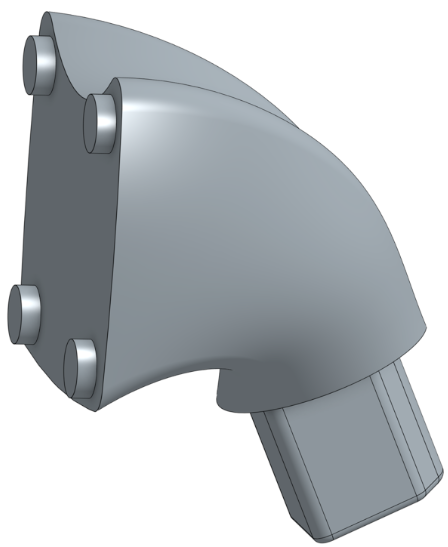
\includegraphics[width = 0.3\textwidth]{Figure/VinkledeHovedbeslag} 
\caption{Illustration af det 3D printede vinklede hovedbeslag designet af Karl Damkjær Hansen i forbindelse med projektsamarbejdet.}
\label{fig:VinkledeHovedbeslag}
\end{figure}
\noindent
%
Ved at erstatte det originale beslag, som medfølger robotten, med det vinklede beslag, illustreret på \autoref{fig:VinkledeHovedbeslag}. Den modificerede \textit{Double}-robot illustreres på \autoref{fig:ModificeretDoubleFront}, \autoref{fig:ModificeretDoubleSide} og \autoref{fig:ModificeretDoubleSideClose}.
%
\begin{figure}[H]
\centering
\begin{minipage}{.33\textwidth}
  \centering
  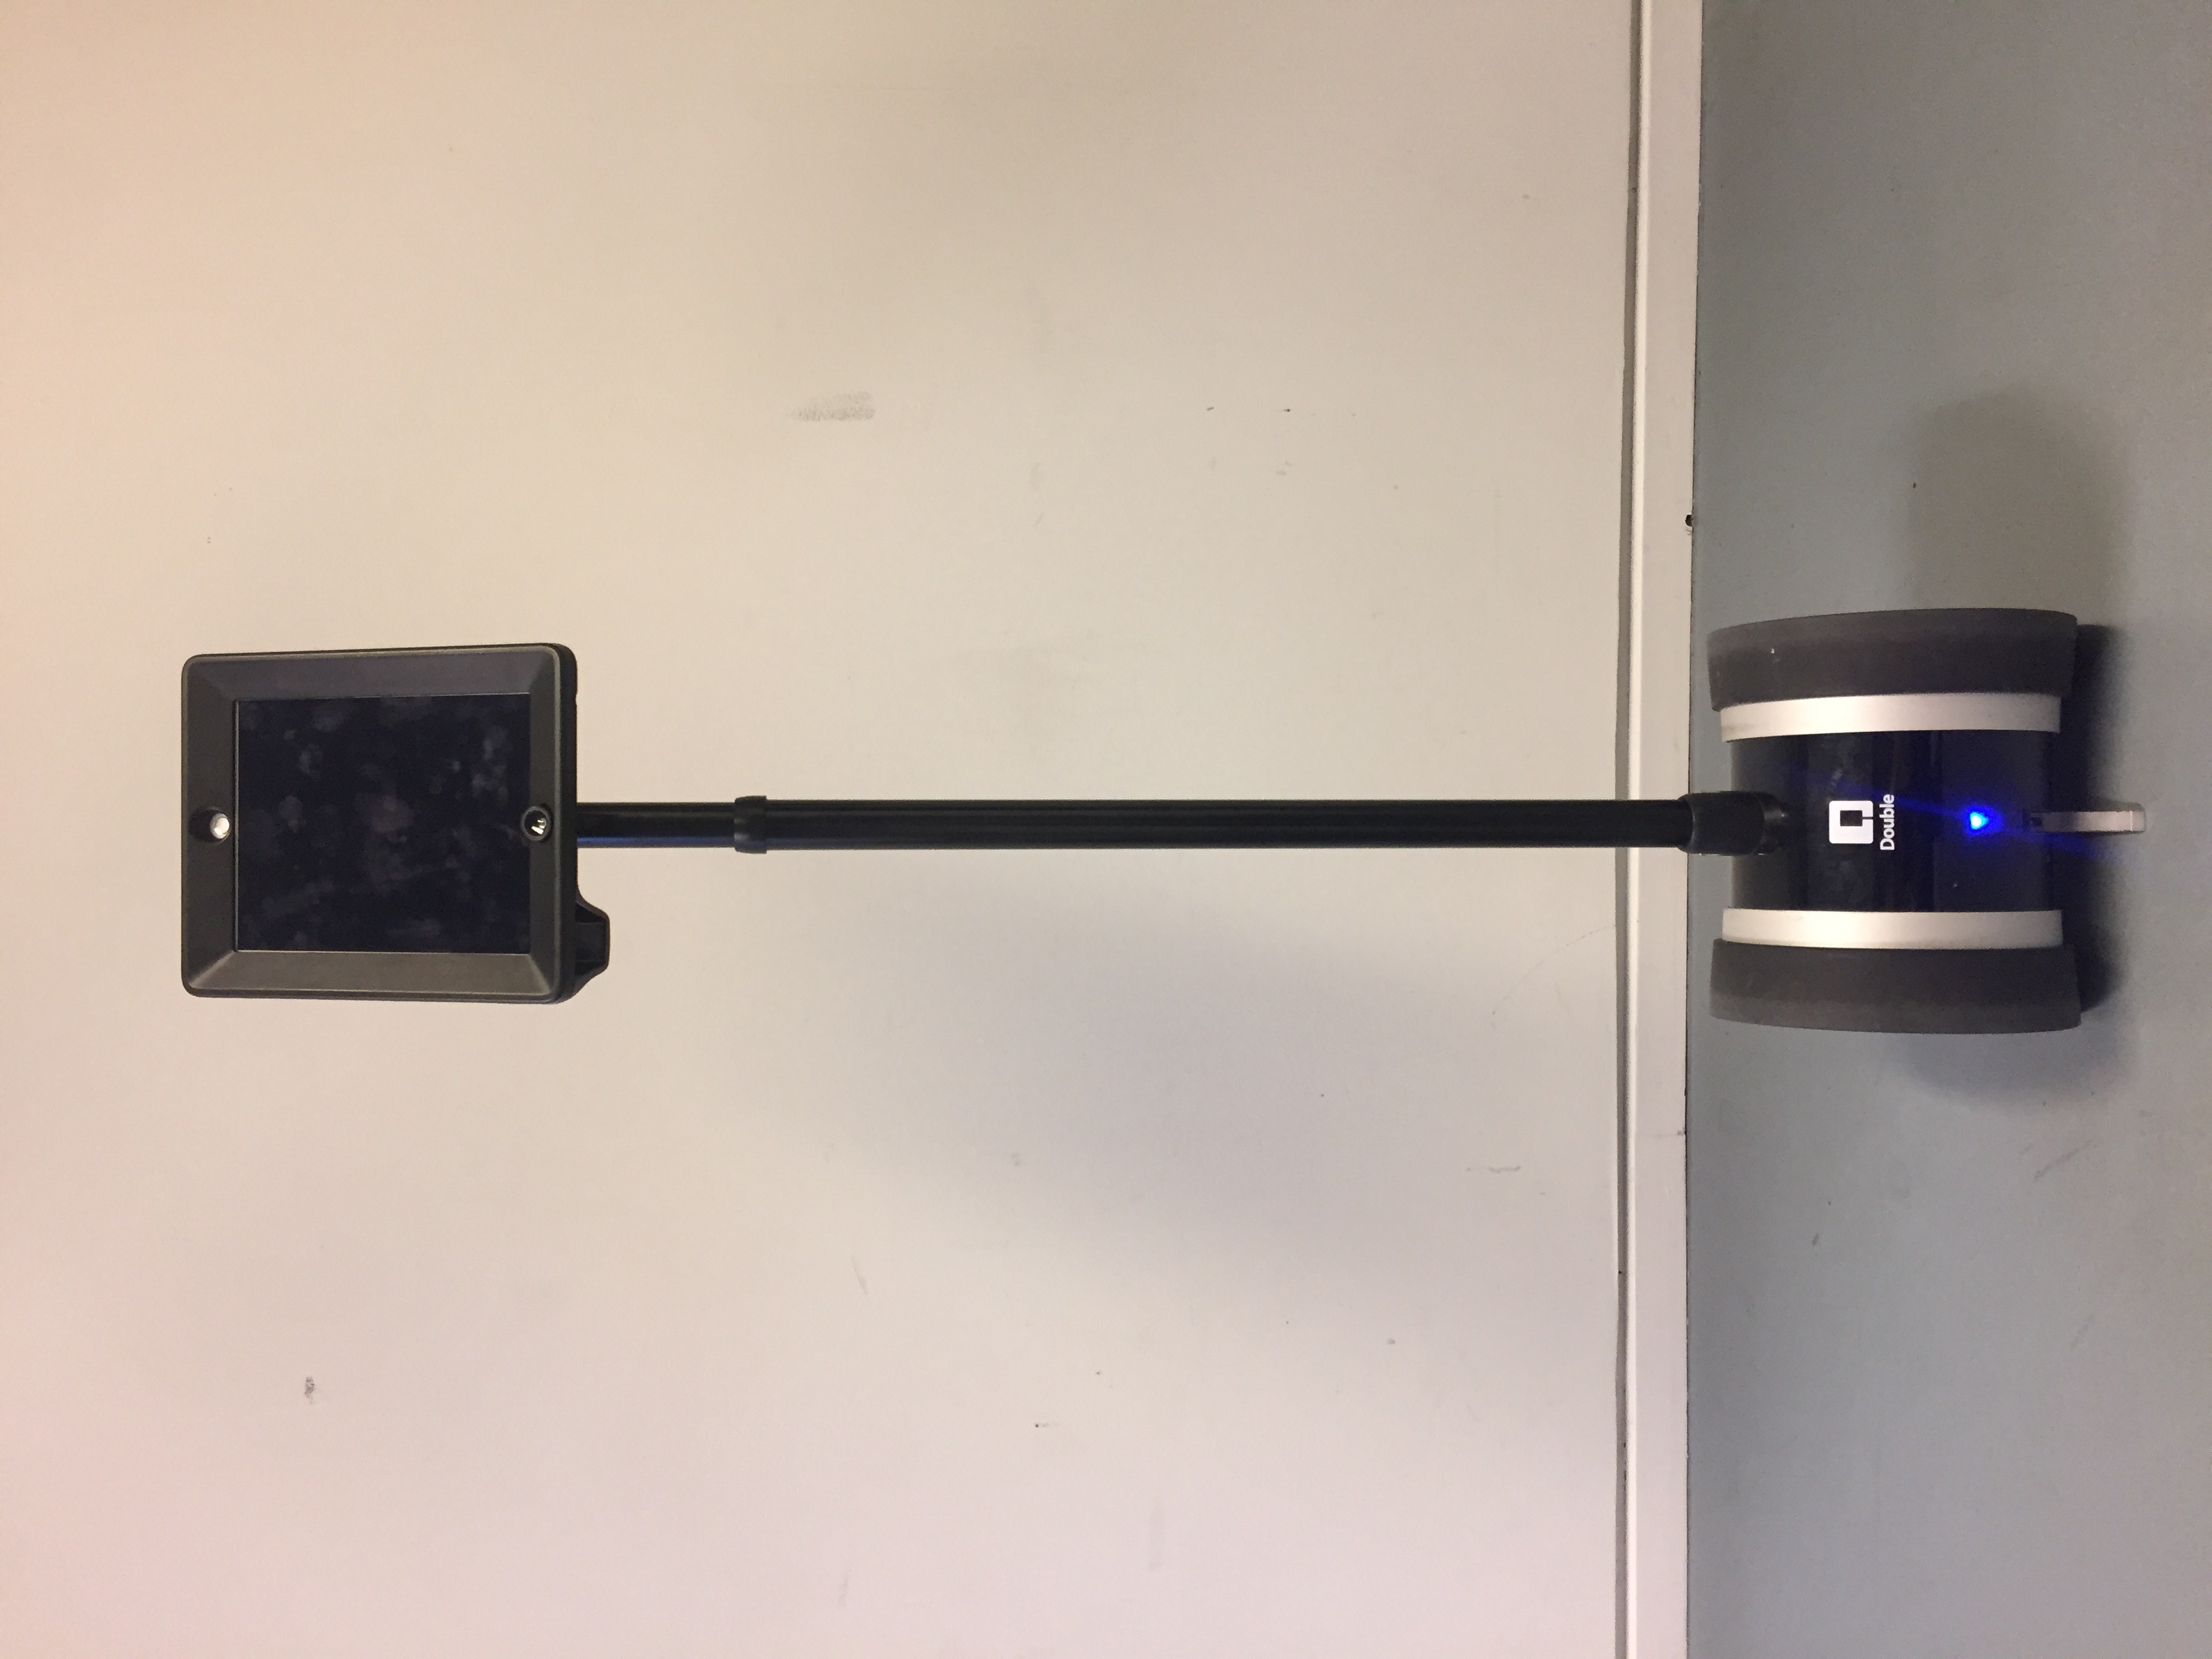
\includegraphics[width=\linewidth, angle =-90]{Figure/ModificeretDoubleFront}
  \caption{Front.}
  \label{fig:ModificeretDoubleFront}
\end{minipage}%
\begin{minipage}{.33\textwidth}
  \centering
  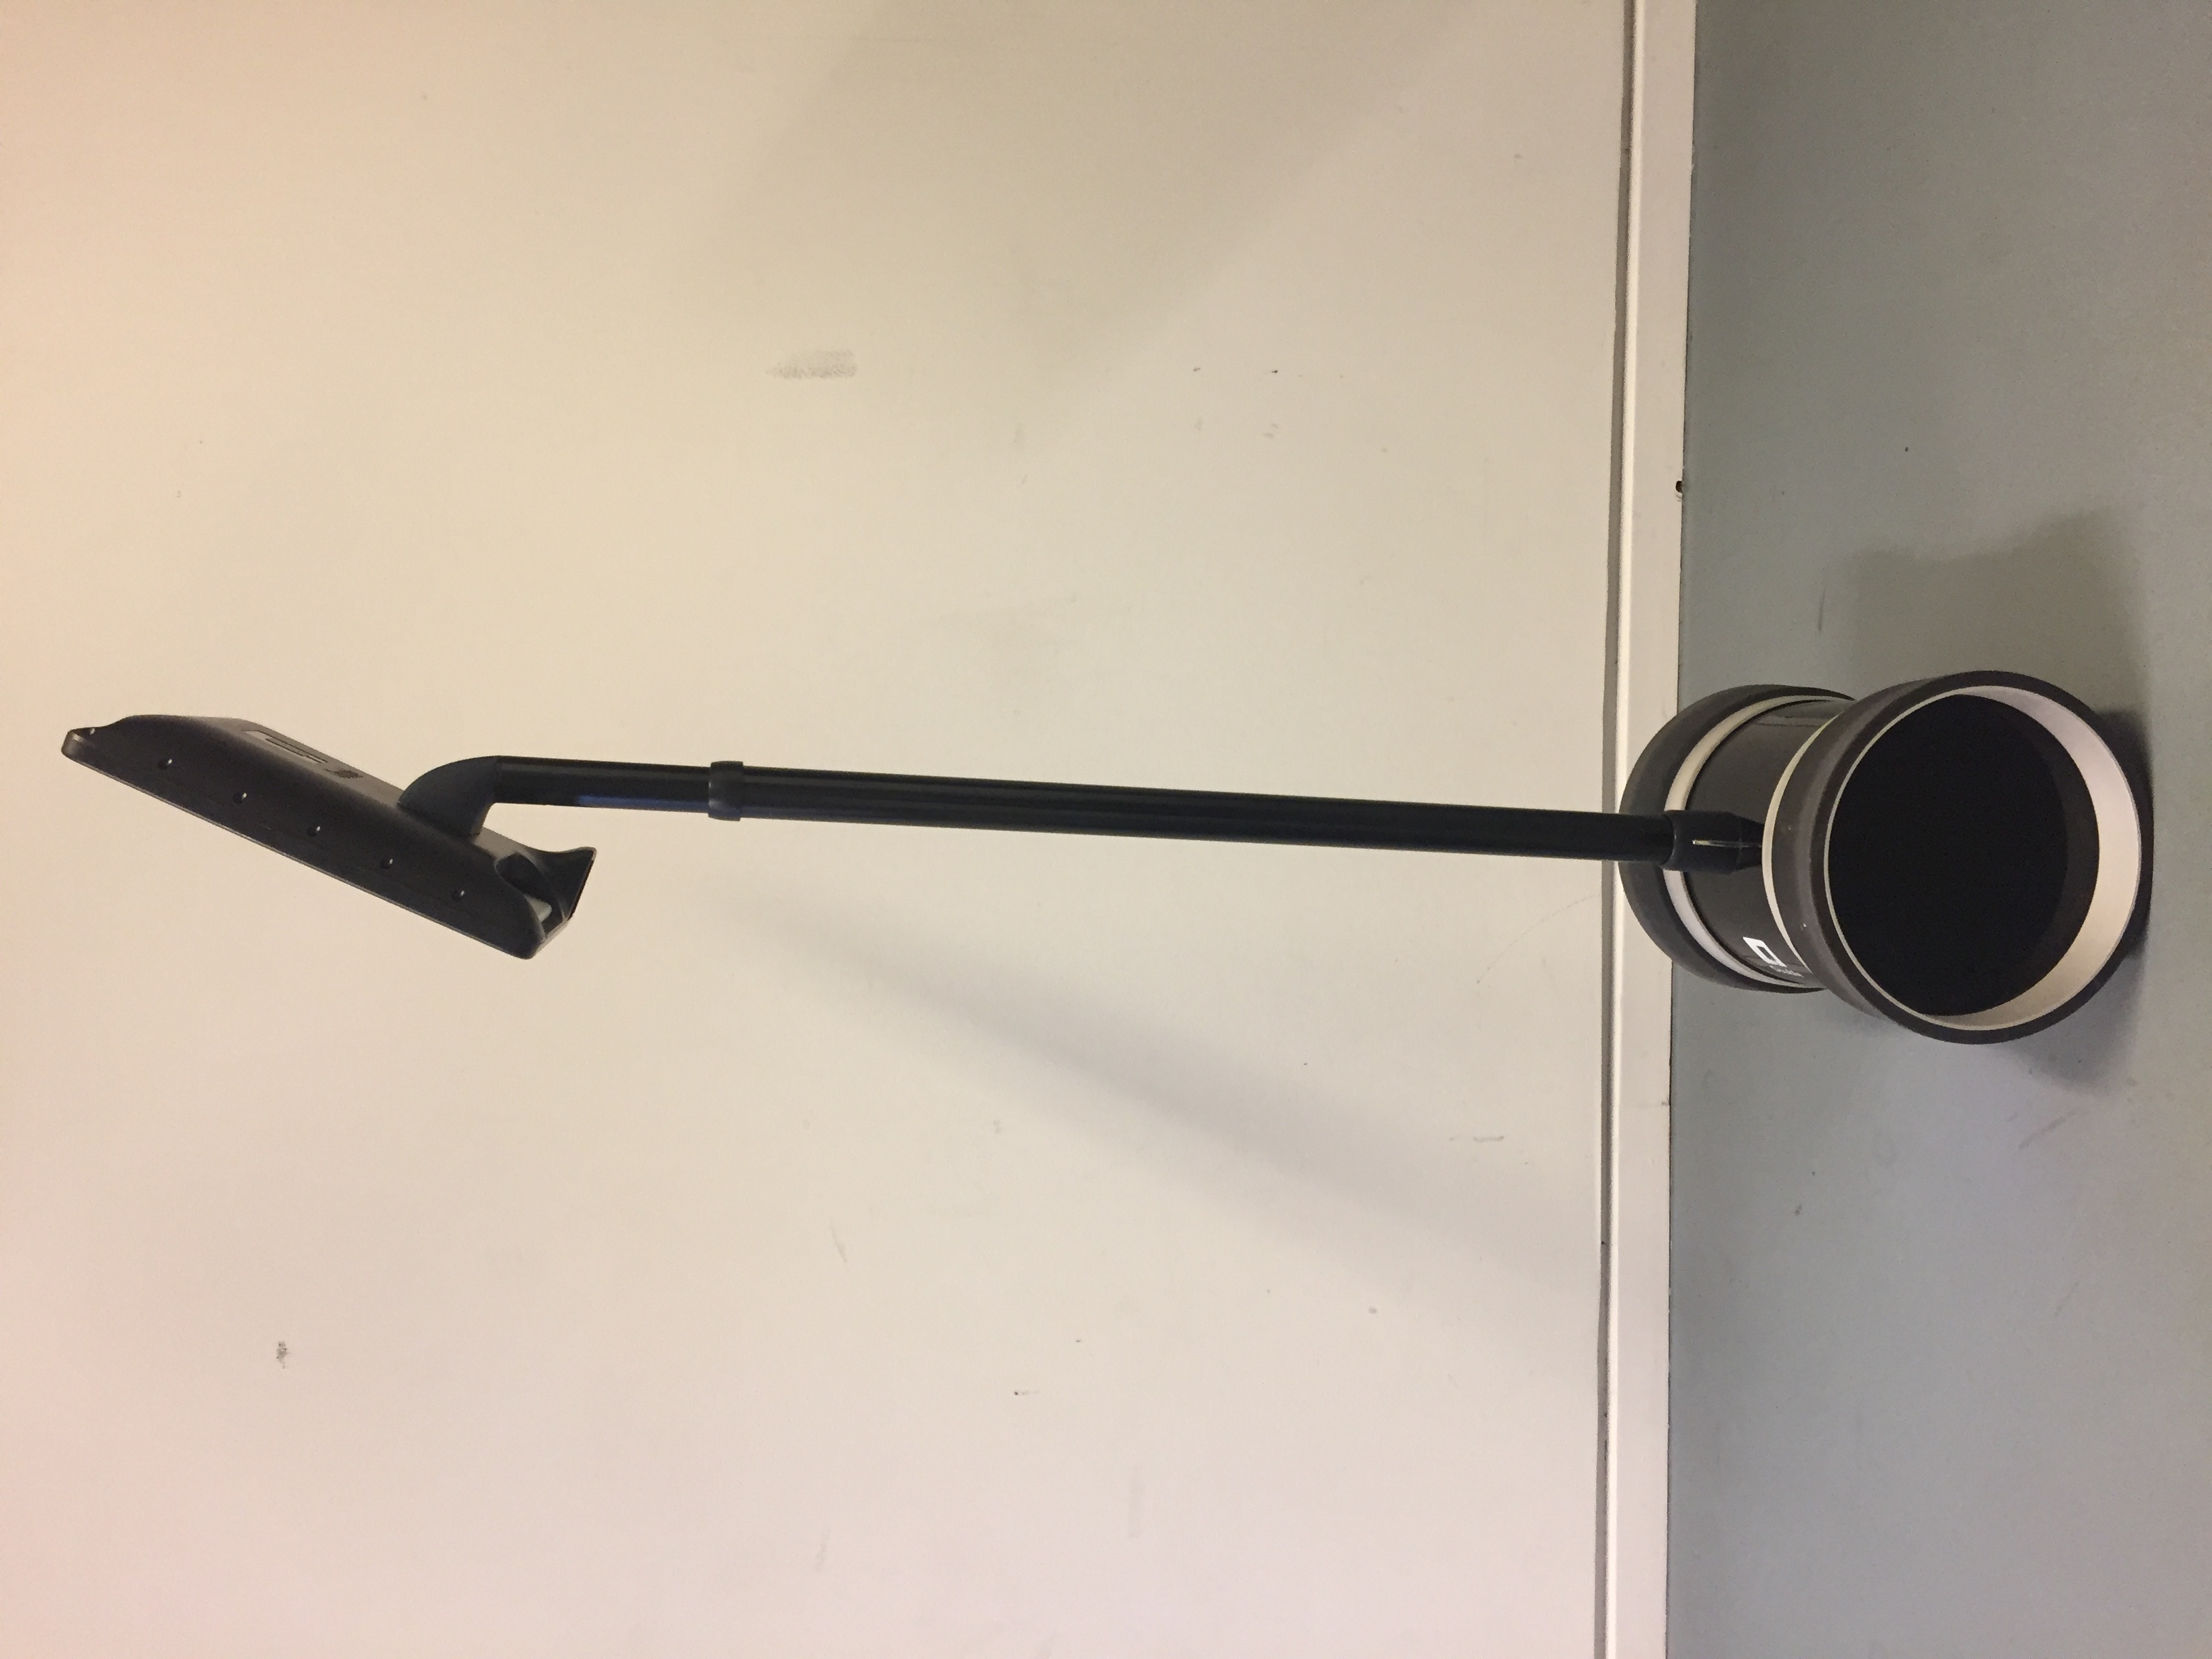
\includegraphics[width=\linewidth, angle =-90]{Figure/ModificeretDoubleSide}
  \caption{Profil.}
  \label{fig:ModificeretDoubleSide}
\end{minipage}
\begin{minipage}{.33\textwidth}
  \centering
  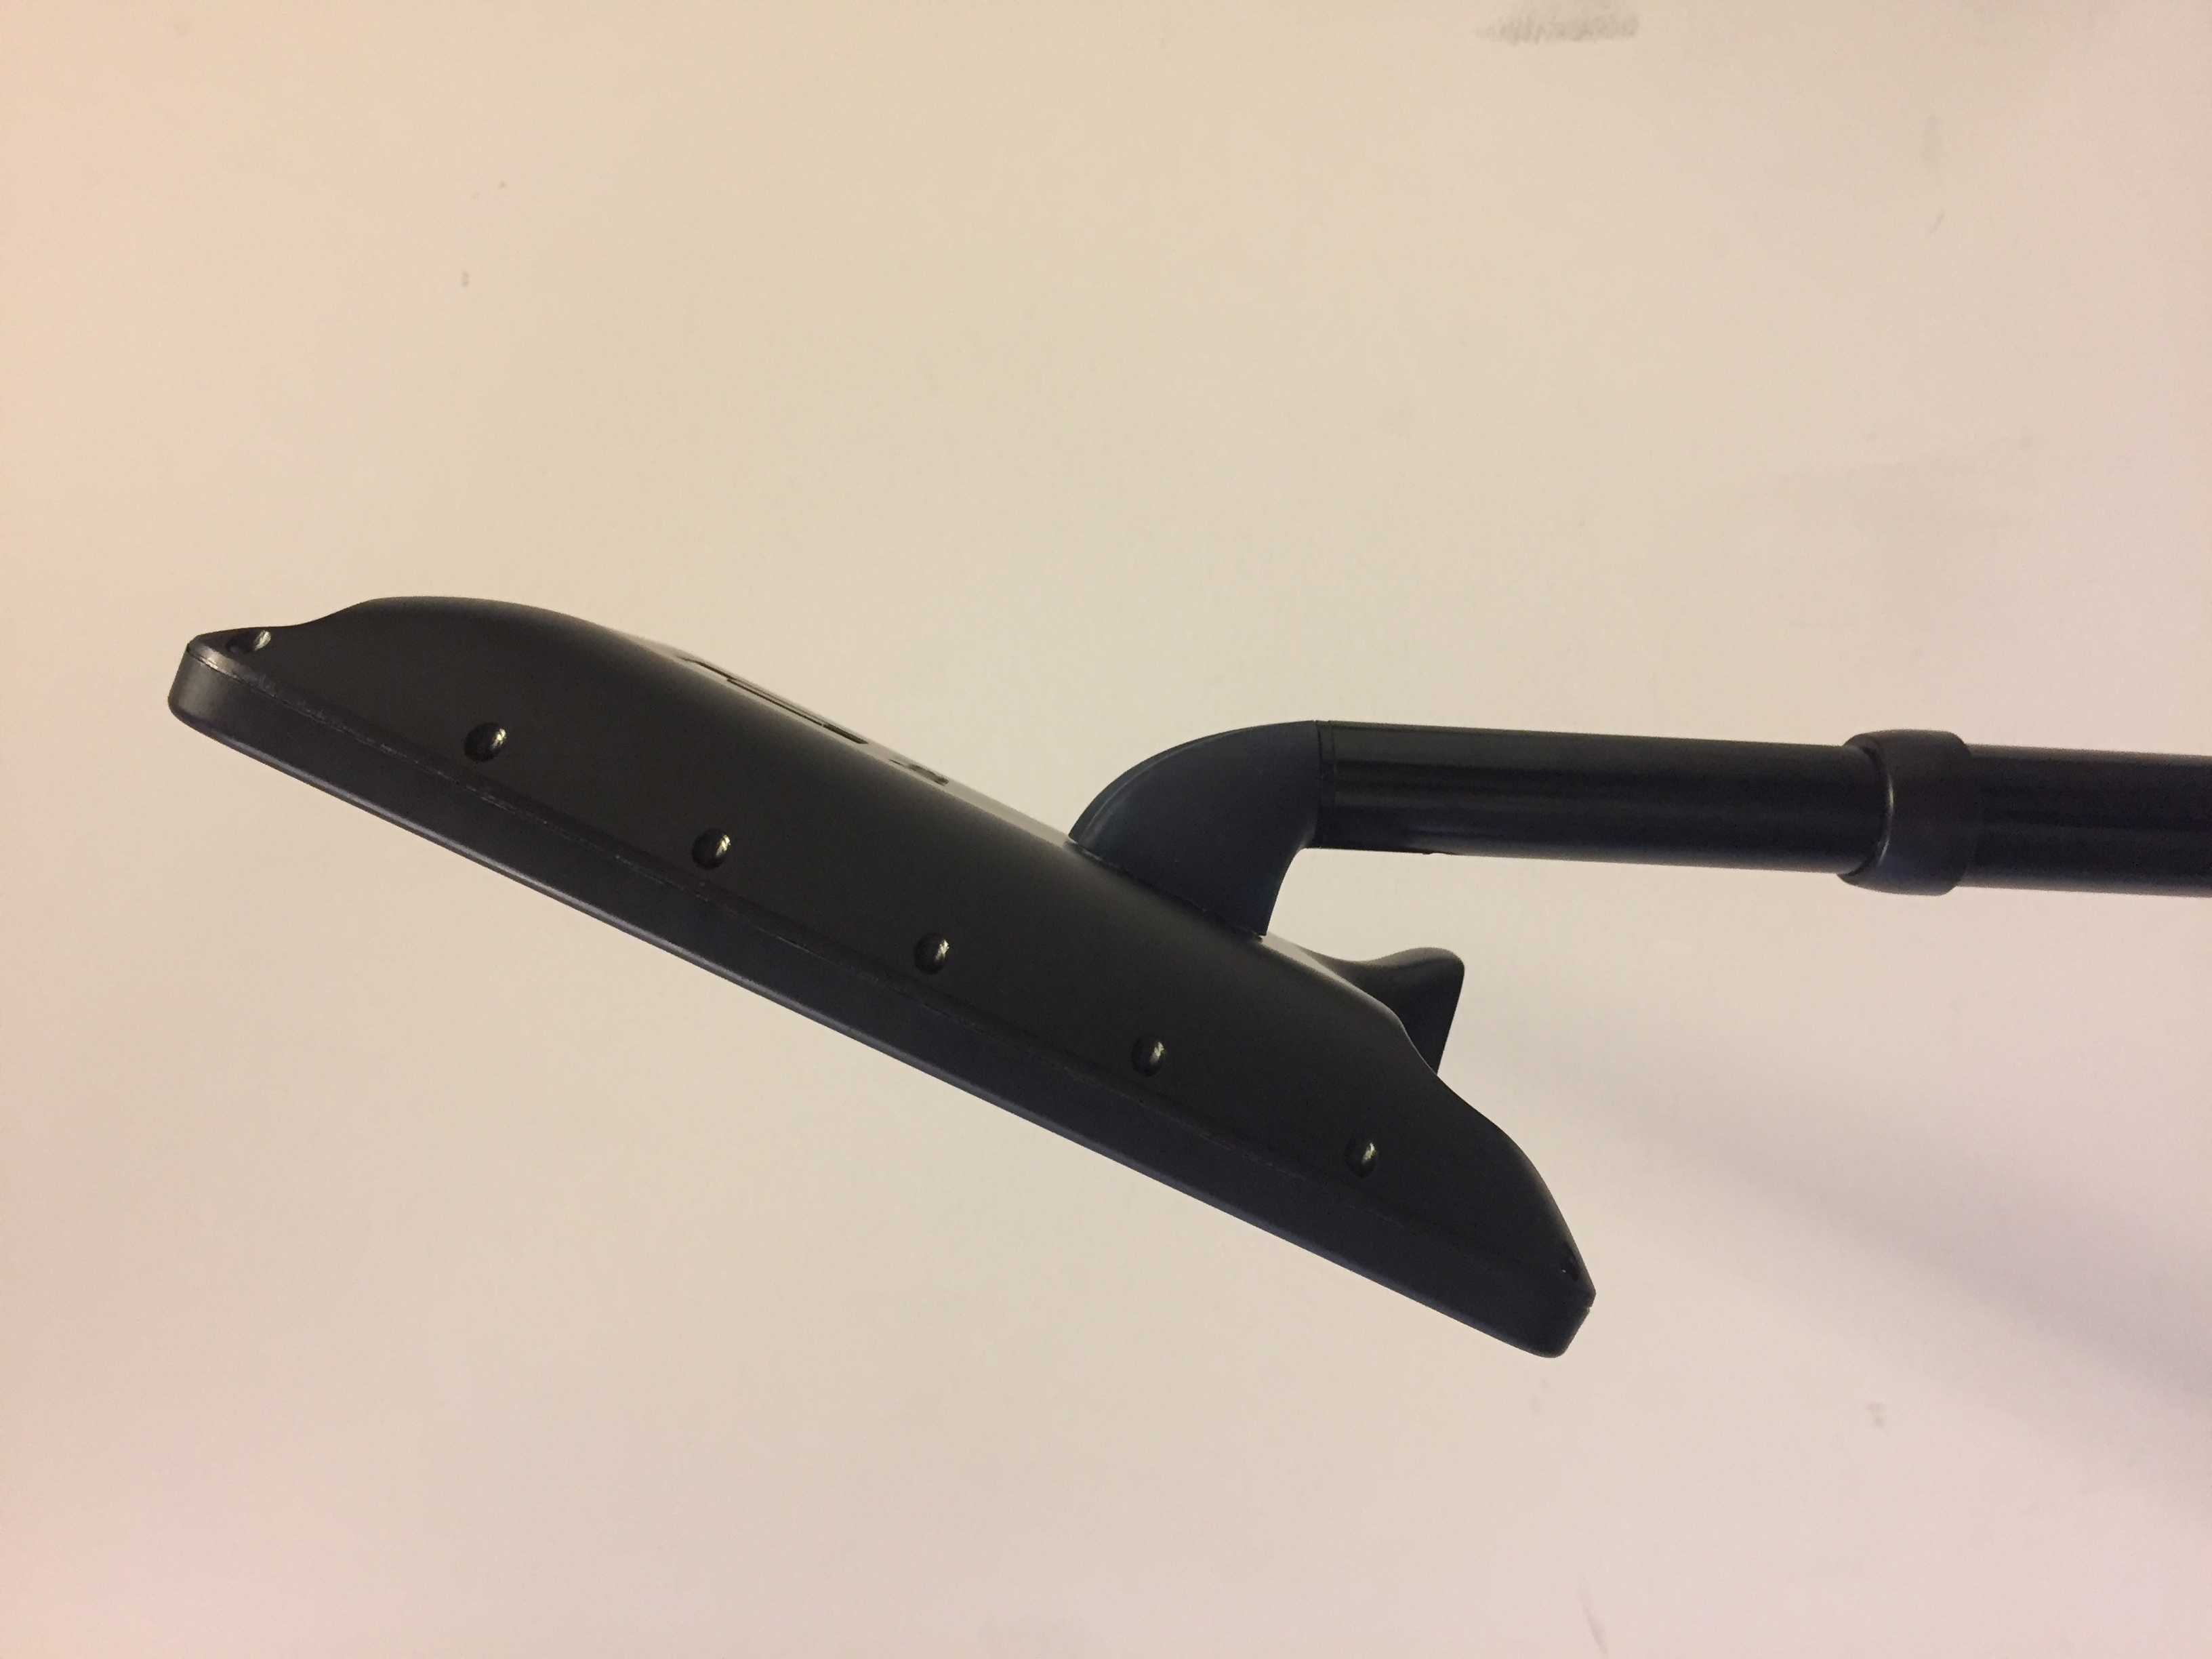
\includegraphics[width=\linewidth, angle =-90]{Figure/ModificeretDoubleSideClose}
  \caption{Profil nært.}
  \label{fig:ModificeretDoubleSideClose}
\end{minipage}
\end{figure}
\noindent
%
Robot styren får tildelt en computer med interadgang. Det er særligt vigtigt at robot styrens computer har interadgang da den skal kommunikere med robotten, hvorfor det kan være nødvendigt at oprette et lukket netværk, eksempelvis ved at lave internetdeling fra ens egen telefon. Igennem \textit{Double}s egen hjemmeside er det muligt at uploade linket til \textit{wireframen}. Observatørerne får tildelt notespapir og kuglepen eller blyant. Lydoptageren anvendes af testlederen til at optage den auditive respons fra testpersonerne, der vælges at lydoptagelsen foretages på en af projektgruppens telefoner. Spørgsmålene i interviewet printes til testlederen.
%

\subsection*{Fremgangsmåde}
\label{Fremgangsmaade}
%
Så snart en af de rejsende befinder sig i det aftalte område vil robotten henvende sig ved at køre hen til den rejsende og spørger om den kan hjælpe dem med at finde rundt i Aalborg Lufthavn. Svarer testpersonen \textit{Ja} vil der efterfølgende ganske kort stå, på skærmen, hvad formålet med testen er: At undersøge menneskers interaktion med robotter. Derefter har testpersonen mulighed for selv at vælge hvad robotten skal hjælpe dem med. Uanset hvad testpersonen beder om hjælp til vil det ende med at robotten opfordre testpersonen til at følge efter. Istedet for at følge testpersonen det rigtige sted hen følger robotten testpersonen hen til testlederen, som tager over. 

Inden samtalen drejes ind på interview spørgsmålene skal testlederen sørger for at give testpersonen tilstrækkelig information omkring testen til at testpersonen kan give et mundtligt samtykke, som tillader at der kan optages lyd. Som nævnt vil der undervejs blive taget noter både før testpersonen er i kontakt med testlederen og efter når de to konverserer. \blankline
%
Da det er robotten, som har stået for rekrutteringen og der ikke har været en mennekse-menneske interaktion før robotten følger testpersonen hen til testlederen, vil de første spørgsmål vedrøre testpersonens førstehåndsindtryk dels af hvordan robotten henvendte sig til testpersonen og dels af hvordan det var at interagere med robotten. Undervejs i samtalen vil robot styren sørger for at robotten køre rundt på forskellige måde, både i forhold til hastigheden, afstanden og højden på robotten vil blive ændret løbende. Det forventes at det er med til at få testpersonerne til at kommentere på netop robottens bevægelse. 

Under debriefingen vil testpersonen blive spurgt om alder og hvor ofte de rejser, hvor kønnet noteres af en af observatørerne.\blankline      
%
Trykker den rejsende derimod \textit{Nej} for ikke at deltage i undersøgelsen, ønsker robotten personen god rejse og forlader stedet og venter til at en ny rejsende befinder sig i området.



     
